
\begin{figure}[h]        
    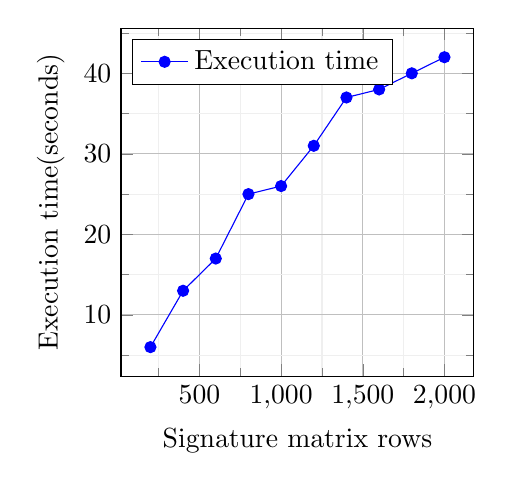
\begin{tikzpicture}
    \begin{axis}[
        xlabel=Signature matrix rows,
        ylabel=Execution time(seconds),
        height=6cm,
        width = 0.5*\textwidth,
        grid = both,
        minor tick num = 1,
        major grid style = {lightgray},
        minor grid style = {lightgray!25},
        legend cell align = {left},
        legend pos = north west
    ]
    
    \addplot[color=blue,mark=*] coordinates {
    	(200, 6)
    	(400, 13)
    	(600, 17)
    	(800, 25)
    	(1000, 26)
    	(1200, 31)
    	(1400, 37)
    	(1600, 38)
    	(1800, 40)
    	(2000, 42)
    };
    
    \legend{Execution time}
    \end{axis}
    \end{tikzpicture}
    
    \caption{\normalfont The time required to search for the most similar query grows as the signature matrix's row count rises.}
    \label{fig:signature_matrix_rows_time}
\end{figure}
